\documentclass[11pt,a4paper]{report}

\usepackage{graphicx}
\usepackage{amsmath}
\usepackage[backend=bibtex]{biblatex}
\graphicspath{{./images/}}
\addbibresource{sources.bib}

\title{Indoor positioning using the comparison of digital imagery to 3D models}
\date{2015}
\author{Jason David Russell}

\begin{document}

\maketitle
\thispagestyle{empty}

\pagenumbering{roman}
\setcounter{page}{0}

\newpage
\chapter*{Plagiarism Declaration}
	\addcontentsline{toc}{chapter}{Plagiarism Declaration}
	\begin{enumerate}
		\item
			I know that plagiarism means taking and using the ideas, writings, works or inventions of another as if they were one's own. I know that plagiarism not only includes verbatim copying, but also the extensive use of another person's ideas without proper acknowledgement (which includes the proper use of quotation marks). I know that plagiarism covers this sort of use of material found in textual sources and from the Internet.
		\item
			I acknowledge and understand that plagiarism is wrong.
		\item
			I understand that my research must be accurately referenced. I have followed the rules and conventions concerning referencing, citation and the use of quotations as set out in the Departmental Guide.
		\item
			This assignment is my own work, or my group's own unique group assignment.
			I acknowledge that copying someone else's assignment, or part of it, is wrong, and that submitting identical work to others constitutes a form of plagiarism.
		\item
			I have not allowed, nor will I in the future allow, anyone to copy my work with the intention of passing it off as their own work.
	\end{enumerate}
	Jason David Russell

\newpage
\chapter*{Acknowledgements}
	\addcontentsline{toc}{chapter}{Acknowledgements}
	I acknowledge everything.

\newpage
\chapter*{Abstract}
	\addcontentsline{toc}{chapter}{Abstract}
	This paper investigates the viability of a new indoor positioning system which is to make use of the comparison of digital imagery to 3D models. An example scenario would be a person wishing to know which room they are in within a building. A 3D model of the building exists. The person takes a few photographs of her surroundings, the photographs are then compared to the 3D model and the result is presented to the person. The main focus of this paper is on the matching of the images to the 3D model.

\newpage
\tableofcontents

\newpage
\listoffigures

\pagenumbering{arabic}
\setcounter{page}{0}

\newpage
\chapter{Introduction}
	\section{Subject of the Report}
		This report concerns the viability of an alternate indoor positioning method. The method involves comparing a photograph to a 3D interior model in order to determine the location of the photographer. 3D interior models are becoming more and more prominent. New technological advancements and techniques are making it cheaper, quicker and easier to generate interior 3D models. Combine the recent prominence of 3D interior models with the ubiquity of camera equipped smart phones and a new indoor positioning system presents itself. This system depends on the matching of a photograph to a 3D interior model in order to locate the photographer. Thus, the primary focus of this paper is on the matching of a photograph to a 3D interior model.
	
	\section{Objective}
		The objectives of this report are therefore to do something.
		
	\section{Research questions}
		Some questions here.
	
	\section{Plan of Development}
		This report begins by looking at work related to indoor positioning systems. Following on from that, the alternate method will be proposed. Thereafter results of investigations will be presented and discussed.

\newpage
\chapter{Related Work}
	In the sections to follow, existing indoor positioning systems will be discussed. Two main branches of technologies will be covered, namely radio and non-radio technologies.
	
	\section{Radio technologies}
		Any wireless technology can in theory, be used for positioning. Three main techniques exist, each one will be briefly outlined below. The sections to follow will look at existing systems which employ these techniques.
	
	\subsection{Time of arrival}
		\begin{figure}[h!]
			\centering
			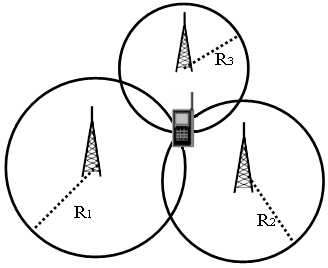
\includegraphics[width=0.6\textwidth]{time_of_arrival}
			\caption{Time of arrival}
		\end{figure}
		Time of arrival (or time of flight) is the travel time of a radio signal from a single transmitter to a single remote receiver. The basic observable is time. A Distance can be directly calculated using the known propagation velocity of signals with the basic observable time. Location can then be determined using multi-lateration. This requires a setup of at least one receiver and three transmitters or vise versa.
		Required with such systems is the synchronization of clocks between receivers and transmitters.
		Time of travel systems suffer greatly from effects such as multi-path.
		\cite{k._pahlavan_wideband_1998}
	
	\subsection{Received signal strength indication}
		\begin{figure}[h!]
			\centering
			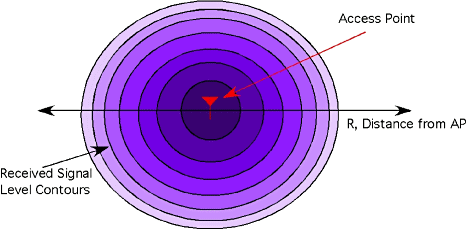
\includegraphics[width=0.6\textwidth]{rssi}
			\caption{RSSI}
		\end{figure}
		Received signal strength indication is a measure of the power level received by a sensor. Because of how radio waves propagate, distance can be approximated between a transmitter and receiver based on the relationship between the transmitted and received signal strength. Multi-lateration can be used to determine locality of a sensor.
	
	\subsection{Angle of arrival}
		\begin{figure}[h!]
			\centering
			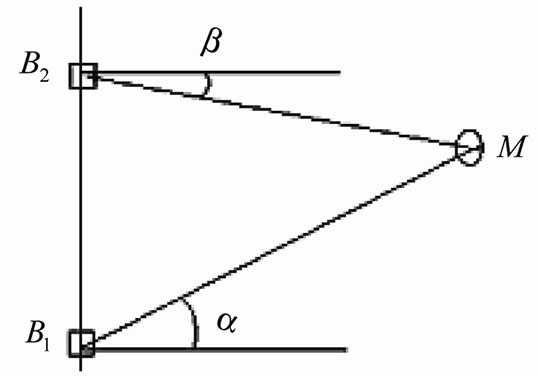
\includegraphics[width=0.6\textwidth]{angle_of_arrival}
			\caption{Angle of arrival}
		\end{figure}
		Angle of arrival is the angle from which a signal is received at a receiver. Angle of arrival is typically determined by using the time difference of arrival between multiple antennas in a sensor array. Position is determined using multi-angulation.
		Angle of arrival systems also suffer from effects such as multi-path.
	
	\subsection{Wi-Fi based systems}
		Wi-Fi based technologies are based on measurements such as TOA (time of arrival), TDOA (time difference of arrival) and DOA (direction of arrival). However these techniques are severely impaired when line of sight is not achievable. These techniques also suffer due to objects such as walls and floors and other objects which attenuate and reflect the signals, directly affecting accuracies.
	
		An alternative Wi-Fi based geolocation method has been explored which makes use of relative signal strengths between transmitters and receivers. So instead of measuring the time or angle of signals, the signal strength is used to determine location. This negates many of the above mentioned deficiencies. A similar system has been employed by animal trackers with directional antennas.
		\cite{yongguang_chen_signal_2002}
	
	\subsection{Blue-tooth systems}
		Blue-tooth positioning works by using proximities, as opposed to angulation or lateration. As such, exact locations are not attainable using these techniques. Instead, the system acts more as a geofence and works by determining which node a device is currently connected to in order to determine the location of the device.
	
		Apple has developed a protocol called iBeacon. This protocol makes use fo Blue-tooth proximity techniques in order to enable smart devices to perform actions when in close proximity to iBeacon.
		\cite{_everything_????}
	
	\subsection{Choke point concepts}
		Choke point systems work by locating and indexing tagged objects in order to track them. The concept works by passing tagged objects though a choke point (or gate), the choke point will then have a sensor which detects the tagged object passing through the gate. Many choke point sensors work with passive radio-frequency identification (RFID) tags which do not report distances or signal strengths.
		\cite{reza_investigation_2008}
	
	\subsection{Grid concepts}
		Grid concepts employ a dense network of low-range receivers arranged in a known pattern. A tagged object will be sensed by only a few nearby, networks receivers. By determining which receivers and tag is sensed by, a rough approximation of the location of the tagged object can be made.
	
	\subsection{Others}
		Various other systems exist but will not be discussed further. These include ultra-wide band (UWB), infra-red (IR), visible light communication, and ultrasound.
	
	\section{Non-radio technologies}
		Non-radio technologies which can be used for indoor positioning will be discussed below. These systems can provide increased accuracy at the expense of increased costs of equipment and additional installations.
	
	\subsection{Magnetic positioning}
		Magnetic positioning takes advantage of the way iron in buildings affects the Earth's magnetic field. The iron in buildings creates local variations in the Earth's magnetic field which can then be sensed by compasses to map indoor locations.
		\cite{supreeth_sudhakaran_geospatial_2014}
	
	\subsection{Inertial measurements}
		Inertial measurement units (IMUs) can be carried by an object in order to track the objects path through space. IMUs measure acceleration and orientation along three orthogonal axis using accelerometers and gyroscopes. Position can be determined by double integration of the acceleration measurements - this is a form of dead reckoning. Dead reckoning is the process of calculating ones current location by using previously determined positions with estimated speed and orientation over some time. This yields relative position estimations. Dead reckoning is subject to what is known as drift which is an accumulation of errors. Due to the susceptibility of IMUs to drift, they are often used in conjunction with other positioning systems in order to correct for this drift.

\newpage
\chapter{Method}
	There are two main requirements for this alternate indoor positioning method. The first requirement is to have a 3D model of an environment. The second requirement is a photograph of a scene within that environment. The premise is that the photograph could be matched against the 3D model in order to determine where the photograph was taken within that 3D model, thus locating the photographer. The focus of this paper is on the comparison of the photograph and the model.
	
	The querying of the photograph against the model presents a problem, and that is that the photograph and the 3D model are not intrinsically comparable. So how does one compare an image to a 3D model? A solution to this problem is to create renderings throughout the model and compare these renderings to the photograph. These renderings are themselves images and so this permits the use of advanced and robust image recognition software to perform the matching.
	
	In the following sections, the processes of creating a 3D interior model, taking a photograph and comparing a photograph to renders of the 3D model will be discussed in detail.
	
	\section{Photograph}
		In this alternate indoor positioning system, a photograph will be take by a person who wishes to know their location within an indoor environment. The photo will typically be take from a mobile device such as a smart phone or tablet.
	
	\newpage
	\section{The 3D model}
		3D modelling can be described as the process of developing a mathematical representation of a three dimensional space using specialized software. The product of this process is called a 3D model. A 3D model can be visualized as a two dimensional image through a process called 3D rendering. It is this two dimensional image representation of a 3D model which is utilized in order to perform the comparison to a photograph in this alternate indoor positioning system. In the subsections to follow, the process of creating a 3D model and associated renderings will be discussed and detailed.
		
		\subsection{Model creation}
			3D models can be created automatically or manually. Examples of automatic techniques include structure from motion. Manual creation of 3D models involves construction by hand using advanced computer software such as Blender. In order to accurately model an existing environment, raw data such as measurements or point clouds is needed to serve as a basis for the model creation, it serves as the initial building block for the model. This raw data can be in a variety of forms, this will be discussed in the section to follow.
		
			\subsubsection{Data acquisition}
				In order to create an accurate 3D model of a building, data is required in order to aid the modelling process and serve as a template or reference. This data can come in the form of building plans, measured distances and directions or point clouds etc.
				Creating a model from a point cloud involves creating vertices, lines and faces based on the positions of points in the point cloud.
				Creating a model from building plans or other measurements involves defining model features in terms of parameters. There is a possibility that the measurements or plans do not accurately reflect the real-world environment in which case the model may contain inaccuracies. 
				
			\subsubsection{Data preprocessing}
				\paragraph{Laser scans}
					During a scan, it often happens that a scanner captures points which are irrelevant. These points may include points which are considered unneeded in a particular scan. Typical examples of such cases leading to irrelevant points are people walking through a scan, reflections of the scan laser beam off of surfaces or points from objects which are deemed irrelevant. Point clouds can be cleaned manually by hand, or using automated techniques.
				
					\begin{figure}[h!]
						\centering
						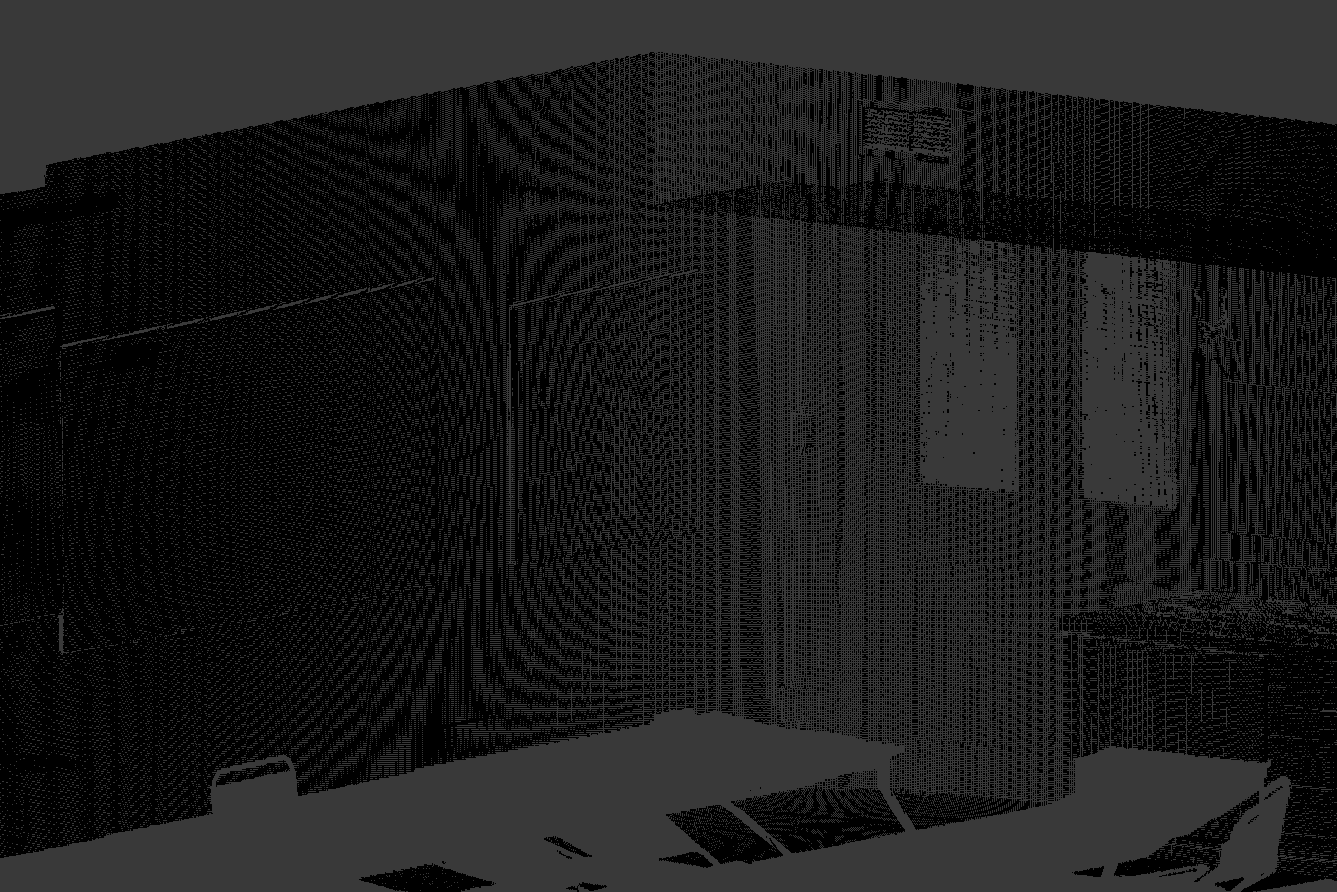
\includegraphics[width=0.9\textwidth]{cleaned_pc}
						\caption{Cleaned point cloud of focus area}
					\end{figure}
				
					The density of the point cloud was also made to be consistent. Due to laser beam divergence, points nearer to the scanner are packed more densely. An operation was performed on the point cloud which ensured uniform point density throughout the cloud. This processes reduces the point cloud's size which in turn makes handling the point cloud less computationally intensive.
					\cite{_selection_????}
				
			\subsubsection{Constructing the model}
				Solid modelling is a consistent set of principles for mathematical and computer modelling of three-dimensional solids which forms the foundation of computer-aided model design. 
				\cite{vadim_shapiro_solid_2001}
				Models are created by using various solid representation schemes. The common aim of these schemes is to organise geometric and topological data in the form of a data structure. 
				
				\paragraph{Pertaining solid representation schemes}
					Boundary representation (B-rep) is a solid representation scheme. It is a method for representing shapes using limits. In boundary representation a solid is represented as a collection of connected surfaces. The surfaces themselves are created using topological items: faces, edges and vertices.
					\cite{hongxin_zhang_introduction_2007}
				
		\subsection{Level of detail}
			In terms of 3D modelling, level of detail refers to how thoroughly real-world features have been modelled and how much those model features resemble their real-world counterparts.
			
			\begin{figure}[h!]
				\centering
				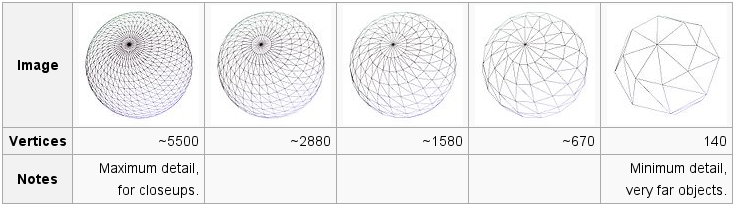
\includegraphics[width=0.6\textwidth]{level_of_detail_example}
				\caption{Level of detail example}
			\end{figure}
			
			The figure above illustrates the concept of level of detail. A sphere has been modelled at various levels of detail, decreasing from left to right.
			
			\subsubsection{Features}
				As many features as possible have been modelled within the area of investigation. This has been done in order to maximise the chance of a high quality match to the photograph as well as to facilitate testing and experimenting with the effect of various levels of detail on the accuracy of a matches. 
				
				This includes the modelling of the wall skirting, the electrical wire conduate, as well as fine details around the whiteboard. 
				
			\subsubsection{Lighting}
				Lighting is a very important component of any 3D model. Lighting can drastically alter the appearance of a model as well as its accuracy. When creating the model for this investigation, a great deal of attention was paid to lighting. Each consideration is discussed in detail below.
				
				\paragraph{Light source}
					The GTL room is illuminated by florescent light panels, each containing three fluorescent tubes. The panels are rectangular with dimensions 0.5m by 1.5m. Additionally, light enters the room from the windows along the north wall, as well as through the glass panels within the door. So there are three sources of light illuminating the room. When modelling light sources, there are a few considerations which need to be made, they are detailed in the paragraphs which follow.
					\subparagraph{Colour temperature}
						The colour temperature of a light source is the temperature of an ideal black-body radiator that radiates light of comparable hue to that of the light source. Colour temperatures are typically statued in the unit of absolute temperature, the Kelvin, with the symbol K.
						\begin{figure}[h!]
							\centering
							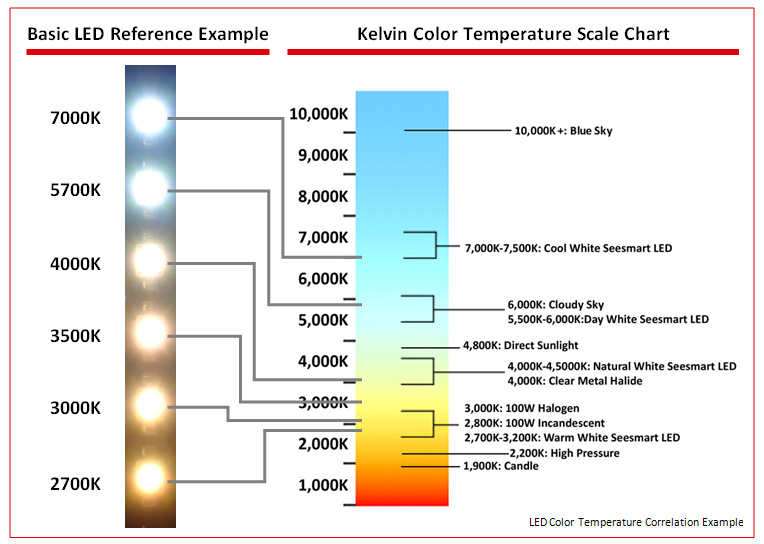
\includegraphics[width=0.6\textwidth]{colour_temperature}
							\caption{Colour temperatures}
						\end{figure}
						The figure above shows how colour temperatures relate to real world scenarios.
				
					\subparagraph{Position of lights}
						In order to accurately replicate shadows and intensities, the lighting in the model needs to be strategically placed and calibrated. The overhead lights have been placed in their respective real-world potions. Three emmisive planes have been placed behind the glass panels of the door area in order to replicate the real-world lighting.
						
						\begin{figure}[h!]
							\centering
							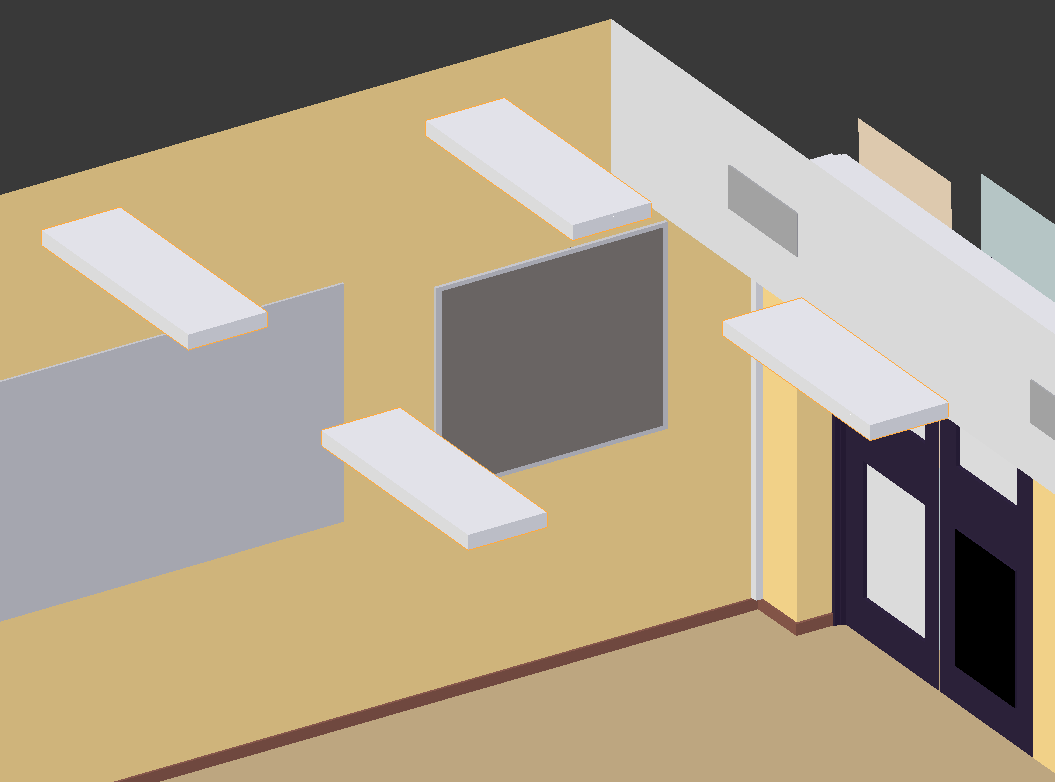
\includegraphics[width=0.6\textwidth]{overhead_lights}
							\caption{Overhead florescent lights}
						\end{figure}
						\begin{figure}[h!]
							\centering
							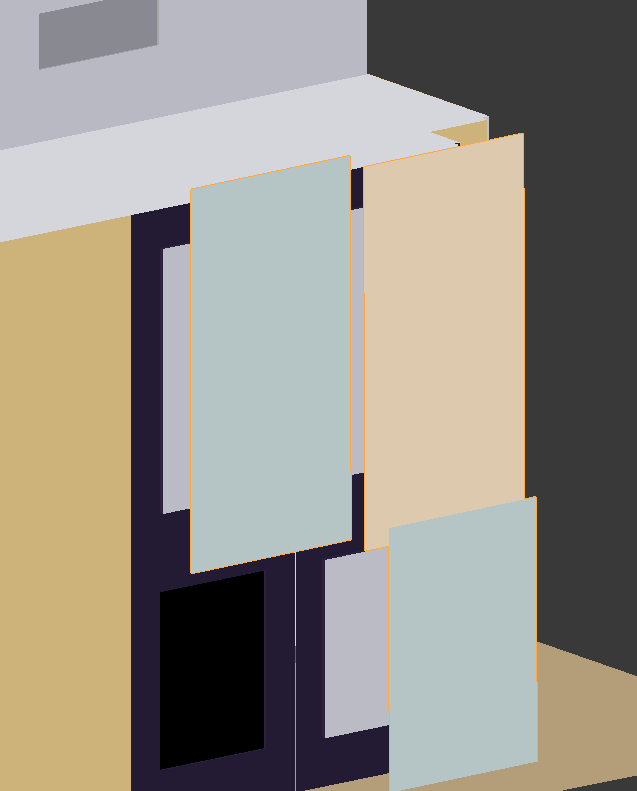
\includegraphics[width=0.6\textwidth]{lights_behind_door}
							\caption{Emmisive planes behind door replicate sunlight}
						\end{figure}
					
					\subparagraph{Light intensity}
						Luminous intensity is a measure of the wavelength-weighted power emitted by a light source in a particular direction. In order to accurately model the real world lighting intensities in the model, each light source was adjusted individually and judged by simple visual inspection. 
						
						One important consideration here is that because the Earth rotates about its axis as well as around the sun, perceived sun light varies. For the sake of this investigation, the lighting conditions were assumed to be that of midday, which was when the photographs for comparison were taken. {{Need more here, clouds affect light etc}}
						
				\subsubsection{Texture}
					Surface finish, also known as surface texture or surface topography, is the nature of a surface as defined by three characteristics of lay, surface roughness and waviness.
					\cite{e._paul_degarmo_materials_2003}
					Particular attention has been paid to accurately representing surface characteristics of as many features as possible in the model.
					The panels in the door are set to be smooth and transparent, replicating the real-world glass panes. 
					The texture of the walls has been adjusted.
					The texture of the floor has been roughened to replicate the carpet.
					The whiteboards are smooth and glossy.
					The gray pin board has a rough texture.
			
			\subsection{Renderings}
				Rendering can be described as the process of generating an image from a 2D or 3D model by means of computer programs. Renders can either be generated in real-time, or pre-rendered. Examples of real-time renderings include 3D video games.
				
				Blender offers three types of renderer engines, Blender, Cycles, and Game renderers. For this investigation, the Cycles renderer was used as it offered superior results.
				
				{{Insert rendered images here}} 
				
				Discus 
			
			\subsubsection{Draft}
				3D model
					Model creation
						data acquisition
							data from laser scan -> Point cloud
						data preprocessing
							cleaned point cloud -> removed unneeded points
							uniform density
						constructing model from raw data
							Intro to solid modelling
							Automated techniques failed
							Boundary rep
							Created model manually with blender + PC
					Model level of detail
						intro to LOD
						elements (degree of detail)
							include conduate, wall plugs, white-board seams etc
						lighting/shadows
							position of lights and shadows, type of lights
						texture
							rough texture for carpet, smooth texture for glass panel on door
						image draping
							image draped over air vent
					creating renderings of model
						types of renderers + their differences
						Cycles renderer used
						Discuss render parameters
			
		\section{Comparison of the model and photograph}
			This section deals with the matching of the photograph to the render of the 3D model. In order to facilitate the matching process, a Python program has been created.
			
			OpenCV (Open Source Computer Vision) is a library of programming functions mainly aimed at computer vision. OpenCV was originally developed by Intel in Russia. OpenCV offers a large range of features, including an image processing module, GUI module, camera construction and 3D reconstruction module, a 2D features framework module as well as many others. The 2D features framework (features2d) was used in this investigation to facilitate the comparison of the photograph to the renders. 
			
			The principle here is that there exist algorithms in OpenCV which, provided with a test image and query image, are able to compare the test image within the query image, yielding transformation parameters which relate the test image to the query image.
			
			\begin{figure}[h!]
				\centering
				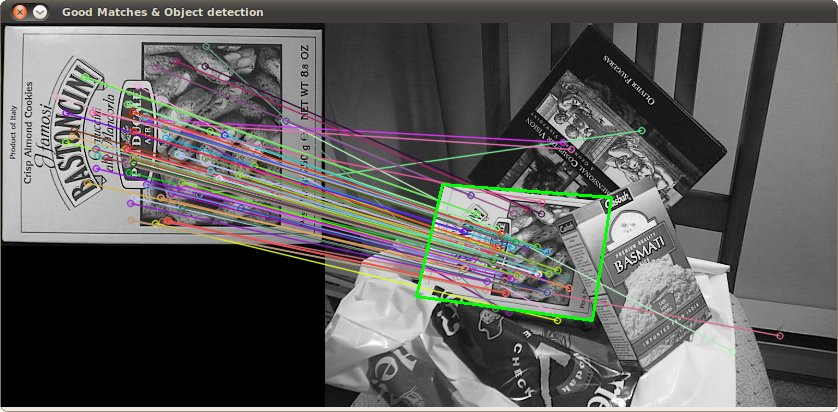
\includegraphics[width=0.9\textwidth]{feature_homography_example}
				\caption{Feature homography}
			\end{figure}
			
			The figure above illustrates the process of comparing a test image to a query image. The figure contains two images, one test image on the left side which is the cover of a rusk box. On the right is the query image. The query image is a more complex scene, which contains the test image inside it. Here, the test image has been detected within the query image, and the algorithm has drawn a green box around where it thinks the test image lies within the query image. This box is defined by a transformation. The process of performing the comparison will be discussed in detail in the sections to follow.
			
			\subsection{Performing the comparison}
				\subsubsection{Key points}
					The first step involved in performing a comparison requires determining what are known as key points within an image. Key points represent specific patterns or features which are unique, can be easily tracked and which can be easily compared.
					
					To provide an example of what key points are, consider the image below:
					
					\begin{figure}[h!]
						\centering
						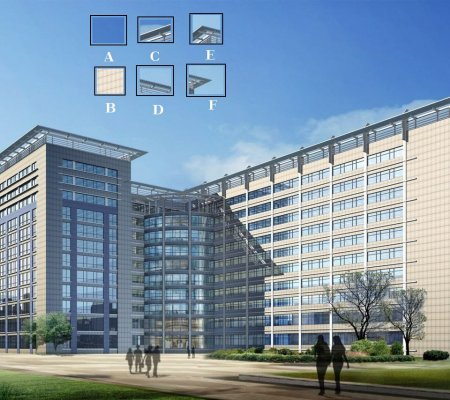
\includegraphics[width=0.9\textwidth]{feature_building}
						\caption{Feature building}
					\end{figure}
					
					The image is of a large building complex. At the top of the image there are six alphabetically labelled blocks. Each block contains a section of the entire image and can be thought of as a key point. We now want to be able to find the exact location of these blocks in the original image. 
					Blocks A and B are flat surfaces, the are spread over a large area and so it is difficult to find the exact location of these blocks.
					Blocks C and D are slightly better in that they are the edges of the building, they could be from anywhere along the edge, but it is still impossible to pinpoint where they are from.
					Blocks E and F are the corners of the building. The locations of these blocks can be exactly found and so these would be good key points as they are unique.
				
				\subsubsection{Finding key points}
					The process of finding key points in an image is called feature detection. On a high level, the process works by looking for regions within an image which have large variation when moved in all directions.
					
					\begin{figure}[h!]
						\centering
						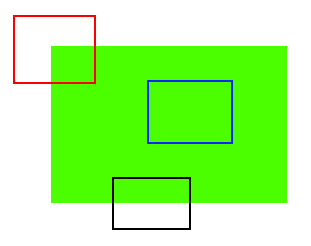
\includegraphics[width=0.9\textwidth]{feature_detection}
						\caption{Feature detection}
					\end{figure}
					
					In the figure above, the green rectangle represents an image and each red, blue and black rectangle represents a region for feature detection. When moving the blue rectangle vertically or horizontally, there is no variation, this represents a poor feature/key point. When moving the black rectangle horizontally, there is also no variation, however when moving it vertically there is. When moving the red rectangle in any direction there is high variation, so this would be a good feature/key point.
				\subsubsection{Describing key points}
					Once key points have been identified, they need to be described. The purpose of describing the key points is to enable the comparison of key points across images. The idea is that a real-world point will have a similar key point description within the images which capture the real-world point.
					
				\subsubsection{Matching key points}
					The final step of the comparison process is that of matching key points. The concept here is that key points from separate images are individually compared against each other. If the similarity of the description of two key points exceeds some threshold, the compared key points are considered a match which would imply that they are the same real-world point.

\chapter{Results}
	\section{Photograph}
		The test photograph for this investigation is of the front door section of the GTL room. The scene consists of a air-conditioning duct on which there is a vent. On the left of the image is a section of a pin board, which contains a number of newspaper clippings. In the centre of the image is the corner of the room. The corner is relatively complex with a number of conduates running to the floor, with an electrical plug box. The blue doors are symmetrical with the exception of the bottom panels where the right hand door as a black ventilation panel. The other three panels are semi transparent glass panes which allow diffused light to enter the room.
		
		The photograph was taken using an iPhone 4S camera, which is actually an eight megapixel Sony Exmor R IMX 145.
		
		\begin{figure}[h!]
			\centering
			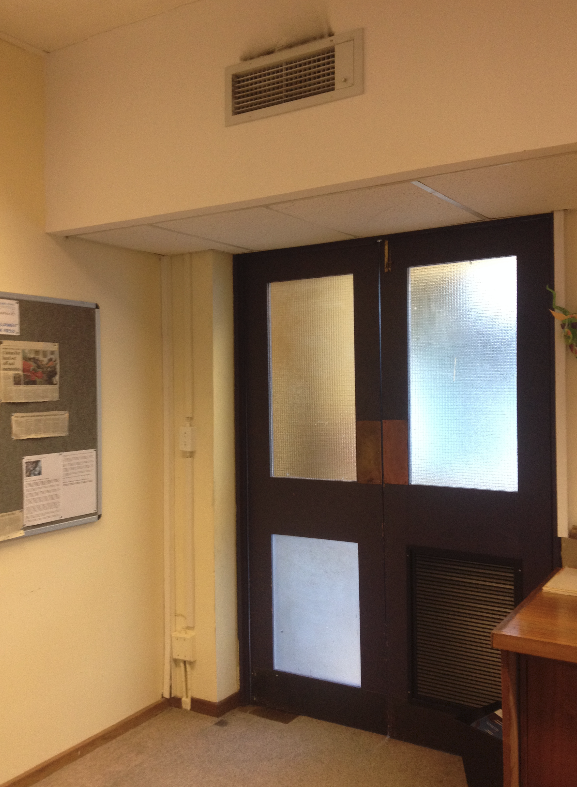
\includegraphics[width=0.6\textwidth]{gtl_door_area}
			\caption{GTL Door area}
		\end{figure}
		
	\section{3D model}
		The front door section of the Geomatics Teaching Laboratory was used as the basis of this investigation. The Geomatics Teaching Laboratory is located on the fifth floor of the Menzies building at UCT. The section under investigation is the south east corner of the room and was selected as there are a number of favourable features which are expected to maximize the chances of a high quality match. Some of these favourable features include the whiteboard, doors, skirting, air-conditioner vents as well as the double lipped corner with a conduate running along an edge. The model was created in an open source software package called Blender.
		\subsection{Model creation}
			\subsubsection{Data acquisition}
				In order to accurately model the scene of interest, a laser scan was conducted. The laser scanner was placed roughly in the centre of the room and a single scan was take. The scan was carried out using a {{laser Scanner model}} at {{laser scanner settings, resolution etc}}. The laser scan yielded a high resolution point cloud which would serve as the basis for the 3D model construction.
				
				{{Insert Point Cloud image}}.
				
			\subsubsection{Data cleaning}
				The point cloud in question was manually cleaned in a software program called CloudCompare. The purpose of cleaning the point cloud is to remove erroneous and superfluous data in order to increase the manageability of working with the point cloud.
	
				The first step cleaning the point cloud involved cutting out the sections which were not to be part of this investigation. This trivial process was performed in a software package called CloudCompare.
				
				{{Image of trimmed PC}}
				
				The second step in cleaning the point cloud involved removing points which existed outside of the rooms confines, such as points outside of the glass panels of the door.
				
				{{Image of cleaned PC}}
 
				The last step in the cleaning process involved making the point cloud uniform in density or resolution. This was done by determining the lowest resolution within the remaining section of the point cloud. This was found to be 7mm and was an acceptable resolution for the scene. So the entire point cloud was eroded to a resolution of 7mm. This removed many superfluous points and considerably reduced the file size of the point cloud.
			
			\subsubsection{Model construction}
				The 3D model in this investigation was created using a solid modelling technique called boundary representation (B-rep). Boundary representation is a solid representation scheme. It is a method for representing shapes using limits or edges. In boundary representation, a solid is represented as a collection of connected surfaces. The surfaces themselves are created using topological items: faces, edges and vertices.
				\cite{hongxin_zhang_introduction_2007}
				Boundary representation was selected as the solid representation scheme as it is very suited to modelling inconsistent or imperfect objects. For example, many objects in the scene appear to be perpendicular, but upon closer inspection it can be seen that very few corners are true, and very few edges are perfectly straight. Boundary representation lends itself to accurately modelling these imperfect which ironically leads to a model which is more accurate, in that the model more accurately represents the real-world features or objects.
				
				The accuracy of the model is an important consideration for this investigation. The model was to be constructed as accurately as possible in order to maximise the chances of obtaining good quality matches, and to serve as a point of further investigation (by investigating the effects of model quality/accuracy on the quality and number of matches).
				
				The software used to create and manipulate the 3D model was Blender. Blender is a free and open-source computer graphics software product. The cleaned point cloud was loaded into Blender and faces were attached to points in order to create the outline of the room, the outline consisted of the four surrounding walls, floor and ceiling. With the extremities constructed, finer and finder features and details were iteratively added to the model, this included the white boards on the walls, the skirting along the bottom of the walls, as well as conduates and electrical plug points, as well as the door section.
				
				\begin{figure}[h!]
					\centering
					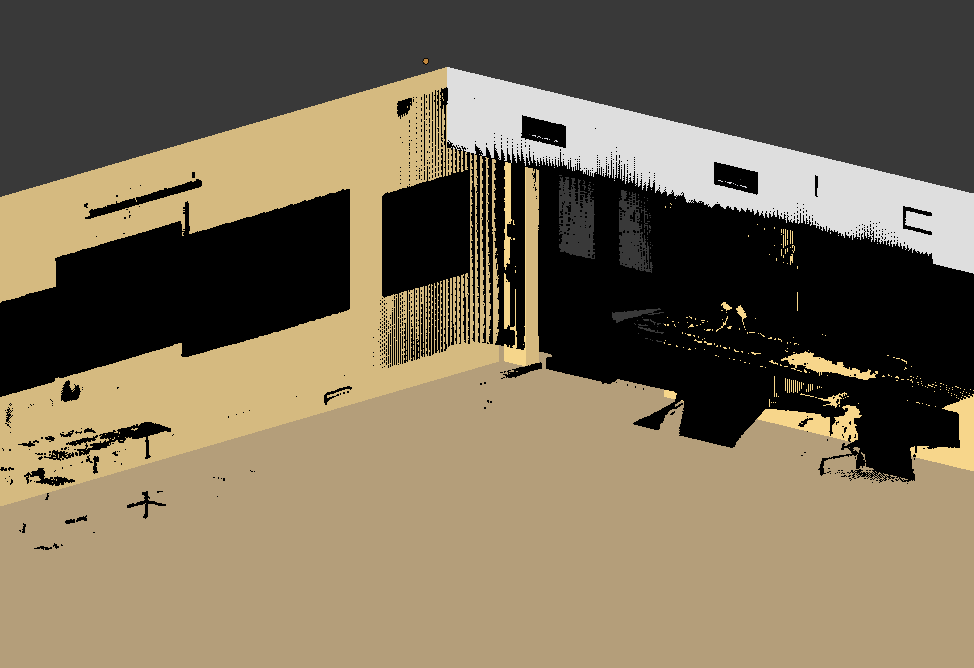
\includegraphics[width=0.9\textwidth]{simple_model_with_pc}
					\caption{Walls, floor and air-conditioning duct modelled from the point cloud}
					\label{fig:simple_model}
				\end{figure}
				
				In figure \ref{fig:simple_model} the walls and floor of the room have been modelled off of the point cloud. 
				
				Detail of the model was iteratively increased by modelling finer and finer details.
				
				\begin{figure}[h!]
					\centering
					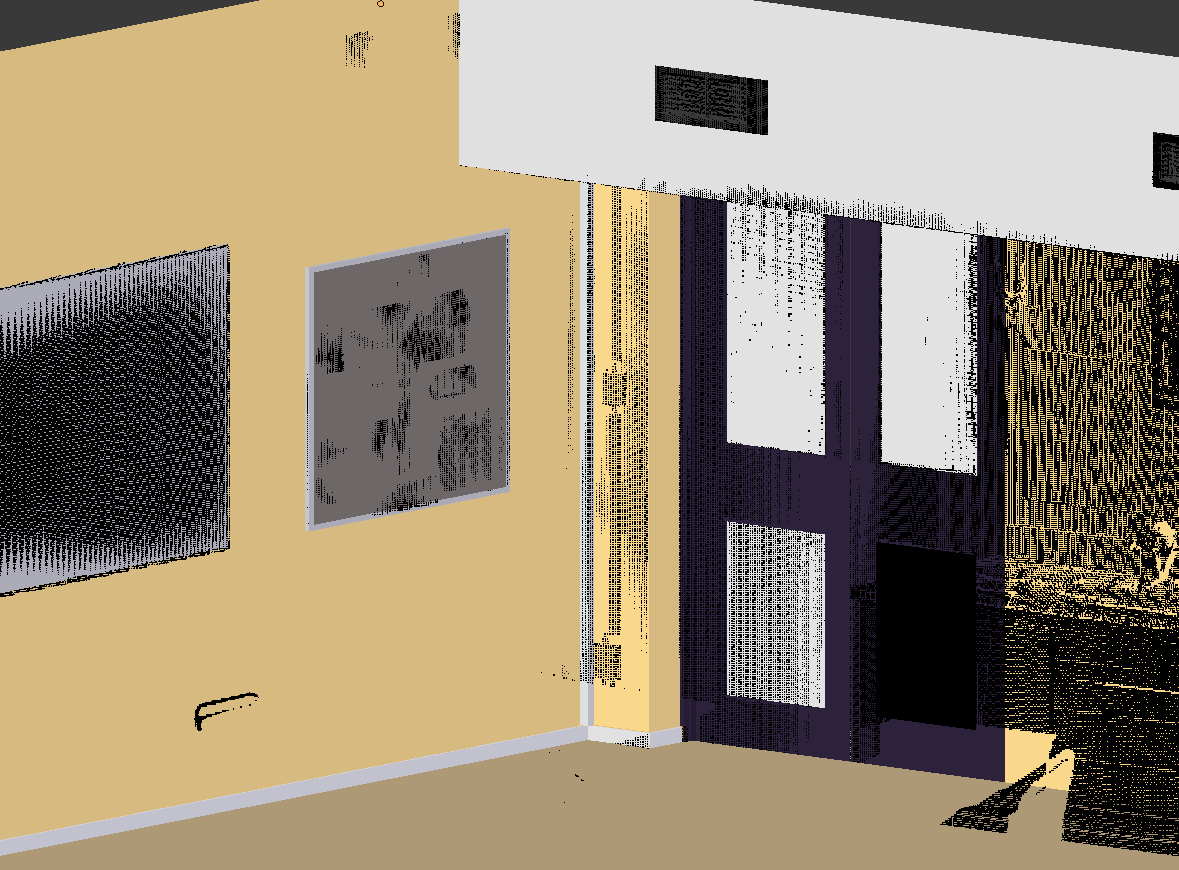
\includegraphics[width=0.9\textwidth]{model_with_increased_detail}
					\caption{Model with increased detail}
					\label{fig:more_complex_model}
				\end{figure}
				
				Figure \ref{fig:more_complex_model} shows the model with increased detail. The skirting board, conduate, door as well as white-boards have now been added. All these features have been modelled from the point cloud and so the model is an accurate representation of the actual room in terms of scale etc.
				
				\paragraph{Lighting}
				Much attention was given to the lighting within the model. This included accurately representing real-world lighting conditions within the model itself. The intensity, colour temperature and locations of light sources are all very important considerations when creating 3D models.
				An important consideration for lighting with regards to this investigation is that lighting can vary. This includes the the variation of natural light throughout the diurnal cycle as well as variations due to weather conditions. Variations in artificial lighting is also important, such variations include lights being on or off, varying brightness etc.
				\subparagraph{Overhead lights}
					Overhead lights consisted of panels of florescent lights uniformly spaced throughout the ceiling. The each panel contained three fluorescent tubes. Theses light panels were reconstructed in the model and mimicked using emmisive planes subtended within a rectangle.
					
					{{Image of modelled florescent lights}}
				
				\subparagraph{External lights}
					In order to accurately model the natural light which penetrates though the glass panes of the door, emmisive planes were placed behind the glass panes of the door section. These emmisive planes were each calibrated in order to best represent real-world conditions of the photograph.
					
					{{Image of emmisive planes behind doors}}
				
				
				
				
				
				
				
				

\chapter{Discussions}

\chapter{Conclusions and future work}

\newpage
\printbibliography

\end{document}